%!TEX root = ../main.tex



\section{Εισαγωγή}

\lettrine[findent=2pt]{\fbox{\textbf{Σ}}}{τα} προηγούμενα κεφάλαια έγινε ανάλυση των κλασικών μεθόδων ρύθμισης ενός PID ελεγκτή και παρουσιάστηκαν οι τρόποι με τους οποίους ο κάθε όρος του ελεγκτή επηρεάζει την απόκριση του τελικού συστήματος. Σε αυτό το κεφάλαιο παρουσιάζεται ο αυτο-ρυθμιζόμενος PID ελεγκτής που αναπτύχθηκε στα πλαίσια της διπλωματικής μου εργασίας. Αρχικά, γίνεται αναφορά στη θεωρία που αφορά την αυτόματη ρύθμιση του ελεγκτή. Στη συνέχεια, παραθέτονται λεπτομέρειες και επεξηγήσεις για τη δομή του προγράμματος που φτιάχτηκε σε LabVIEW έτσι ώστε ο αναγνώστης να καταλάβει τη λογική λειτουργίας του ελεγκτή και τη δομή του προγράμματος.

\section{Θεωρία}

\lettrine[findent=2pt]{\fbox{\textbf{Μ}}}{ε} τον όρο \emph{``αυτο-ρυθμιζόμενος" PID ελεγκτής} ή \emph{αυτόματη ρύθμιση του PID ελεγκτή} εννοούμε μία μέθοδο στην οποία τα κέρδη του ελεγκτή ρυθμίζονται αυτόματα μετά από απαίτηση του χρήστη. Συνήθως, ο χρήστης θα πατήσει ένα κουμπί ή θα στείλει μια εντολή στον ελεγκτή. Μια αυτόματη ρύθμιση του ελεγκτή περιλαμβάνει τα εξής τρία βήματα:

\begin{itemize}
	\item Δημιουργία μιας διαταραχής του συστήματος.
	\item Εκτίμηση της απόκρισης που προκαλεί η διαταραχή.
	\item Υπολογισμός των παραμέτρων του ελεγκτή.
\end{itemize}
Αυτά αποτελούν και τα βήματα που εκτελεί και ένας έμπειρος ελεγκτής όταν κάνει χειροκίνητη ρύθμιση του ελεγκτή. Το σύστημα πρέπει να διαταραχθεί με κάποιον τρόπο έτσι ώστε να εκτιμηθούν οι δυναμικές που το διέπουν. Αυτό μπορεί να γίνει με πολλούς τρόπους όπως, για παράδειγμα, εισάγοντας ημιτονοειδή σήματα, παλμούς ή βηματικές αλλαγές στην είσοδο του συστήματος.

\subsection{Relay Method}
Η μέθοδος που χρησιμοποιήθηκε σε αυτή την εργασία είναι αυτή που στη βιβλιογραφία αναφέρεται ως \emph{``Relay Method"} (δεν υπάρχει ακριβής μετάφραση στα ελληνικά) \cite{astrom}, \cite{vandoren}. Η μέθοδος αυτή βασίζεται, όπως και οι μέθοδοι \emph{Ziegler-Nichols} και \emph{Tyreus-Luyben}, στην απόκριση συχνότητας του συστήματος.

Στην πραγματικότητα, η μέθοδος \emph{Ziegler-Nichols}, όπου το κέρδος που φέρνει το σύστημα στην οριακή ευστάθεια βρίσκεται πειραματικά, είναι μια μορφή αναγνώρισης μοντέλου. Όλες οι τεχνικές ρύθμισης στην πραγματικότητα περιέχουν κομμάτια αναγνώρισης μοντέλου,
αλλά οι πιο δημοφιλείς απλά βελτιώνουν και αποκρύπτουν αυτά τα κομμάτια καλύτερα. Στην ουσία, όλη η διαδικασία ρύθμισης χρησιμοποιώντας τη μέθοδο Ziegler-Nichols γίνεται για να βρεθεί το κέρδος στο οποίο το σύστημα έχει μισό κύκλο καθυστέρηση όταν λειτουργεί σε ανατροφοδότηση. Αυτό είναι που αναφέρθηκε στην Ενότητα \ref{subsec:Ziegle-Nichols Method} ως απόλυτο κέρδος $K_u$ και σχετίζεται με το σημείο όπου η καμπύλη Nyquist του συστήματος κόβει πρώτα τον πραγματικό άξονα, όπως φαίνεται στο Σχήμα \ref{fig:nyquist}.

\begin{figure}[h]
  \centering
  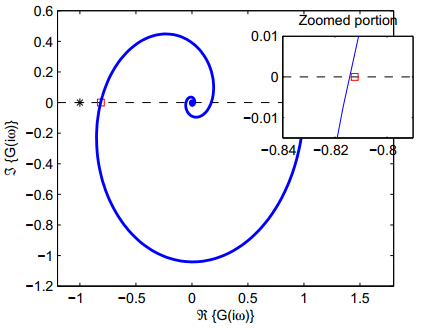
\includegraphics[width=\textwidth]{nyquist}
  \caption{Διάγραμμα Nyquist ενός ανοιχτού σταθερού συστήματος με κάποια καθυστέρηση (deadtime)}
  \label{fig:nyquist}
\end{figure}

Το πρόβλημα με τη μέθοδο αυτή είναι ότι για να βρεθεί το απόλυτο κέρδος, το σύστημα θα πρέπει να φτάσει στα όρια του, με ό,τι αρνητικές συνέπειες μπορεί να επιφέρει αυτό, τόσο στη λειτουργία του όσο και στην κατασκευή του. Η μέθοδος ``Relay" που περιγράφεται εδώ καταφέρνει να βρίσκει πειραματικά τόσο το απόλυτο κέρδος όσο και την απόλυτη συχνότητα του συστήματος. Τα βήματα που ακολουθούνται για την εφαρμογή της μεθόδου είναι τα ακόλουθα:
\begin{enumerate}

\item Προσωρινά, ο ελεγκτής δίνει τη θέση του σε μία μη γραμμική συνάρτηση (στην ουσία είναι on-off	έλεγχος) (Σχήμα \ref{fig:relay}) η οποία εναλλάσσει την είσοδο του συστήματος μεταξύ δύο διακριτών τιμών. Κάθε φορά που η τιμή του σφάλματος $e(t)$ (δηλαδή $setpoint - output$) είναι μεγαλύτερη από το μηδέν η έξοδος του relay στοιχείου είναι $d$. Κάθε φορά που η τιμή του σφάλματος $e(t)$ είναι μικρότερη από το μηδέν η έξοδος του relay στοιχείου είναι $-d$.

\item Αποφεύγοντας την εις βάθος μαθηματική ανάλυση \cite{astrom}, η αντικατάσταση του ελεγκτή με ένα relay στοιχείο, εξαναγκάζει το σύστημα να εκτελεί ταλαντώσεις σταθερού πλάτους και συχνότητας (Σχήμα \ref{fig:relay2}). Η συχνότητα αυτή είναι σχεδόν ίδια με την απόλυτη συχνότητα του συστήματος, ενώ το απόλυτο κέρδος είναι αντιστρόφως ανάλογο του πλάτους της παρατηρούμενης ταλάντωσης.

\item Περιμένουμε η απόκριση του συστήματος να σταθεροποιηθεί σε αμείωτες ταλαντώσεις σταθερής συχνότητας και καταγράφουμε το πλάτος $\alpha$ και την περίοδο $T$.
 
\item Η παρατηρούμενη περίοδος είναι η απόλυτη περίοδος, δηλαδή $T_u=T$, ενώ το απόλυτο κέρδος συνδέεται με το πλάτος $\alpha$ με τη σχέση,
\begin{equation}
K_u = \frac{4d}{\pi\alpha}
\label{eq:Ku}
\end{equation}

\item Έχοντας υπολογίσει το απόλυτο κέρδος και την απόλυτη περίοδο, μπορούν να οριστούν τα κέρδη του PID ελεγκτή με βάση τους Πίνακες \ref{table:zn_method} και \ref{table:tl_method} των μεθόδων Ziegler-Nichols και Tyreus-Luyben αντίστοιχα.

\end{enumerate}

\begin{figure}[h]
  \centering
  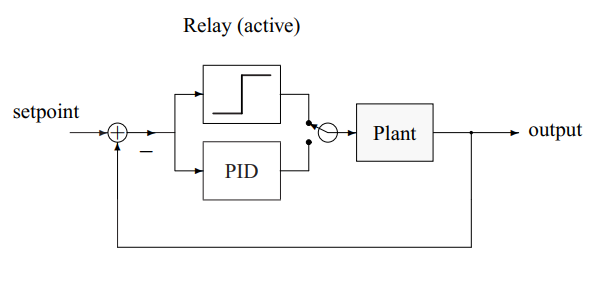
\includegraphics[width=\textwidth]{relay}
  \caption{Δομικό διάγραμμα συστήματος με relay στοιχείο}
  \label{fig:relay}
\end{figure}



Η διαδικασία της αντικατάστασης του PID ελεγκτή με το relay στοιχείο, η μέτρηση του πλάτους και της περιόδου των ταλαντώσεων και ο υπολογισμός των κερδών του ελεγκτή μπορεί να αυτοματοποιηθεί αξιόπιστα. Αυτή η μέθοδος χρησιμοποιείται και σε εμπορικά διαθέσιμους PID ελεγκτές. Σημαντικό πλεονέκτημα της μεθόδου αυτής σε σχέση με τη μέθοδο Ziegler-Nichols είναι ότι το σύστημα δεν χρειάζεται να διεγείρεται στα όρια του. Επειδή το πλάτος των ταλαντώσεων $\alpha$ είναι ανάλογο του πλάτους $d$ του relay, μπορούμε να ορίσουμε το πλάτος $\alpha$ έτσι ώστε οι ταλαντώσεις να μην είναι υπερβολικά μεγάλες και, κατά συνέπεια, επικίνδυνες για το σύστημα ή τον εξοπλισμό.

\begin{figure}[H]
  \centering
  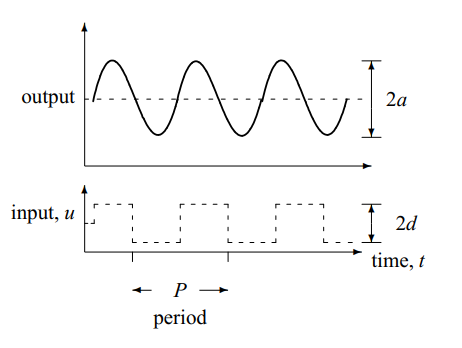
\includegraphics[width=\textwidth]{relay2}
  \caption{Ταλαντώσεις ενός συστήματος υπό συνθήκες ανατροφοδότησης μέσω relay στοιχείου αντί για ελεγκτή.}
  \label{fig:relay2}
\end{figure}

\section{Το Πρόγραμμα}

\lettrine[findent=2pt]{\fbox{\textbf{Σ}}}{την} ενότητα αυτή θα παρουσιαστεί το πρόγραμμα σε LabVIEW που υλοποιεί τον αυτο-ρυθμιζόμενο PID ελεγκτή. Για την καλύτερη οργάνωση του προγράμματος, το κυρίως VI αποτελείται από επί μέρους subVIs που το καθένα επιτελεί διαφορετική λειτουργία του προγράμματος. Σε κάθε υποενότητα λοιπόν θα παρουσιάζεται ένα από αυτά τα subVIs και θα αναλύεται η δομή του καθώς και η λειτουργία που επιτελεί.

\subsection{Το Front Panel και το Block Diagram}

\subsubsection{Front Panel}

Στο Σχήμα \ref{fig:Auto-tuning_PIDp} φαίνεται το front panel του προγράμματος LabVIEW, το οποίο αποτελεί το γραφικό περιβάλλον του αυτο-ρυθμιζόμενου PID ελεγκτή και περιλαμβάνονται όλες οι επιλογές για τη ρύθμισή του.  

\begin{figure}[h]
  \centering
  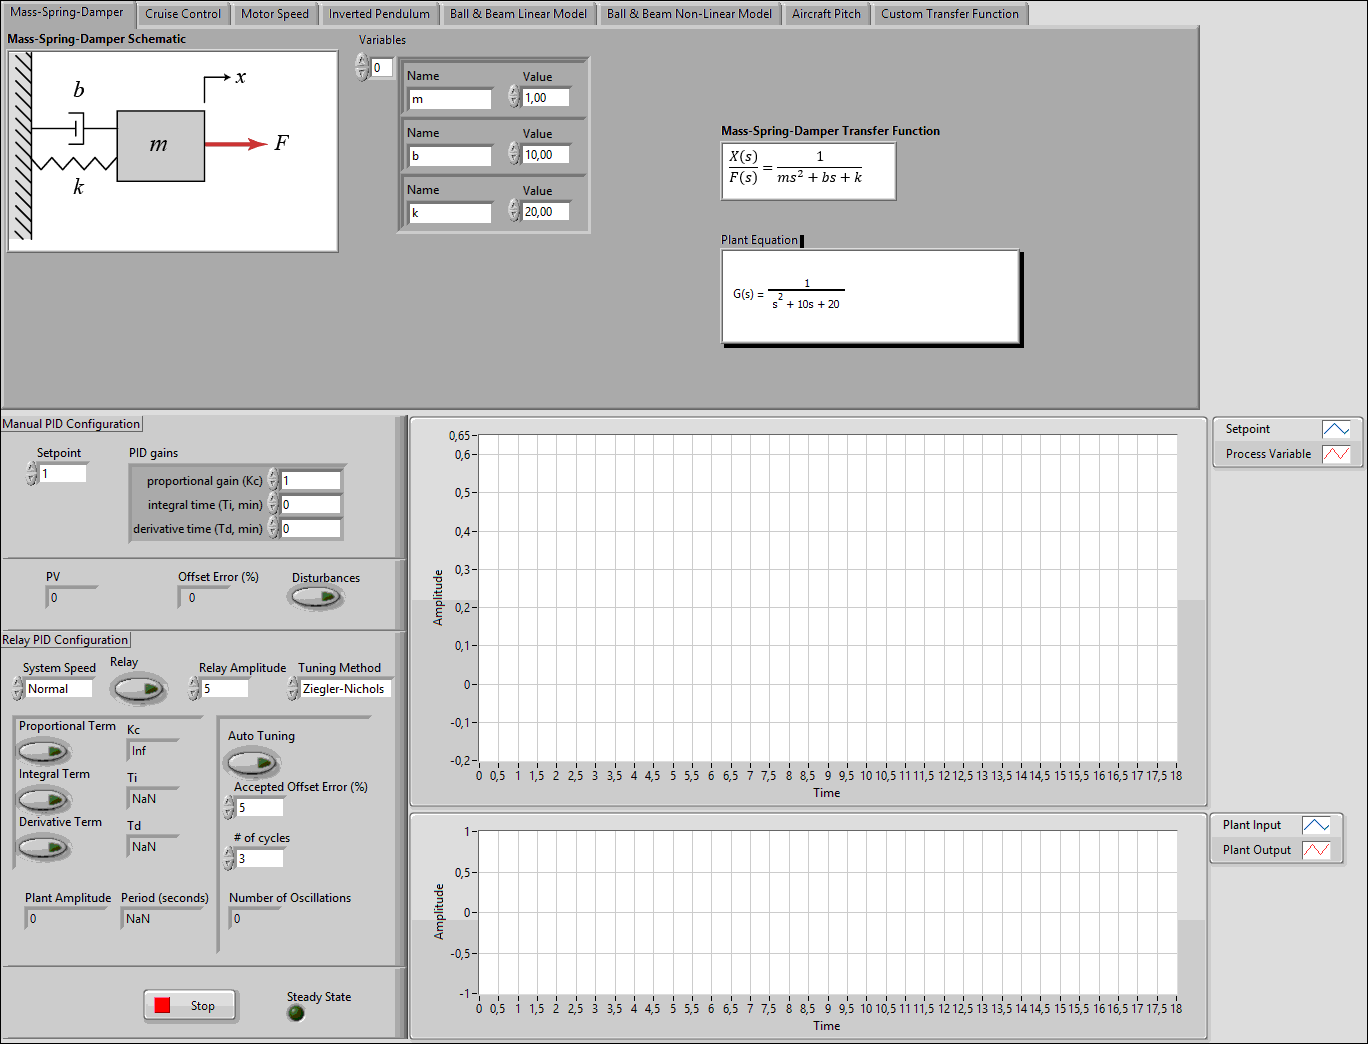
\includegraphics[width=\textwidth]{Auto-tuning_PIDp}
  \caption{Το Front Panel του Αυτο-Ρυθμιζόμενου PID Ελεγκτή}
  \label{fig:Auto-tuning_PIDp}
\end{figure}

Στην κορυφή του front panel φαίνονται τα διαφορετικά φυσικά συστήματα που έχουν αναλυθεί και μοντελοποιηθεί προκειμένου να φανεί κατά πόσο ο αυτο-ρυθμιζόμενος PID ελεγκτής είναι ικανός να ελέγξει αποδοτικά το καθένα από αυτά.

Πιο κάτω, στα αριστερά, βρίσκονται τα κουμπιά ελέγχου του ελεγκτή καθώς και οι δείκτες που δείχνουν την τρέχουσα τιμή της εξόδου του συστήματος αλλά και το ποσοστό του σφάλματος που υπάρχει μεταξύ αυτής και της επιθυμητής τιμής της. Υπάρχουν επιλογές τόσο για χειροκίνητη ρύθμιση των κερδών του ελεγκτή από κάποιον χειριστή, όσο και επιλογές για την αυτόματη ρύθμιση αυτών, με βάση τη μέθοδο relay που περιγράφηκε προηγουμένως.

Στα δεξιά βρίσκονται τα διαγράμματα που θα παρουσιάσουν με γραφικό τρόπο την απόκριση του συστήματος. Το πάνω γράφημα δείχνει ταυτόχρονα τη βηματική απόκριση του κλειστού συστήματος και την επιθυμητή τιμή που θέλουμε να έχει η έξοδος του συστήματος. Το κάτω γράφημα δείχνει ταυτόχρονα την είσοδο και την έξοδο του συστήματος. Αυτό σημαίνει ότι στην περίπτωση που στο σύστημα είναι συνδεδεμένος ο ελεγκτής, το γράφημα αυτό θα μας δείχνει το σήμα ελέγχου και την απόκριση του συστήματος, ενώ αν είναι συνδεδεμένο το relay στοιχείο θα μας δείχνει τον τετράγωνο παλμό που θα παράγει αυτό σε σχέση με τις ταλαντώσεις του συστήματος.

\subsubsection{Block Diagram}

Στο Σχήμα \ref{fig:Auto-tuning_PIDd} φαίνεται ολόκληρο το block diagram. Αυτός είναι ουσιαστικά ``ο κώδικας" του προγράμματος. Όπως έχει αναφερθεί και σε προηγούμενο κεφάλαιο, το LabVIEW είναι περιβάλλον γραφικής γλώσσας προγραμματισμού οπότε οι διάφορες συναρτήσεις του συνδέονται μεταξύ τους με καλώδια μέσω των οποίων περνάνε τα δεδομένα από τη μία συνάρτηση στην επόμενη. 

\begin{figure}[h]
  \centering
  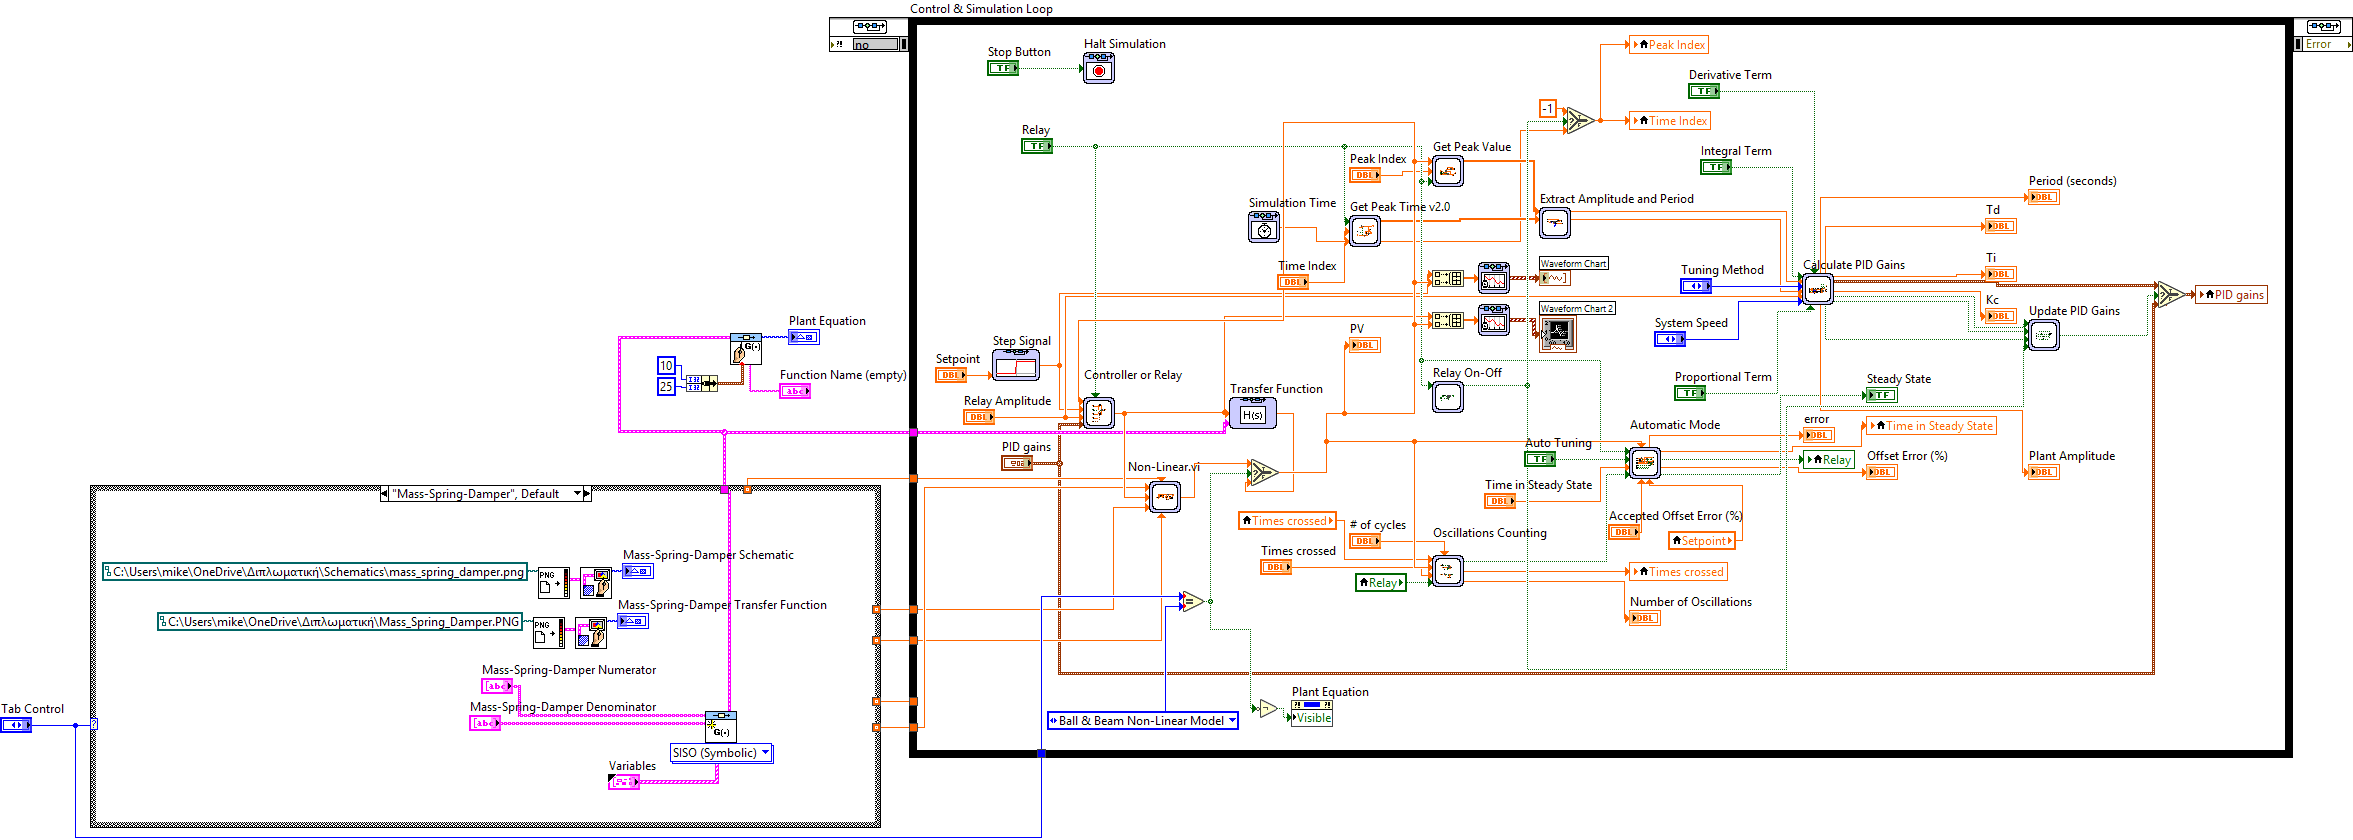
\includegraphics[width=\textwidth]{Auto-tuning_PIDd}
  \caption{Το Block Diagram του Αυτο-Ρυθμιζόμενου PID Ελεγκτή}
  \label{fig:Auto-tuning_PIDd}
\end{figure}

Στη συνέχεια κρίνεται σκόπιμο να αναλυθούν τα επιμέρους κομμάτια του block diagram, το καθένα ξεχωριστά, έτσι ώστε να γίνει κατανοητός ο τρόπος υλοποίησης των διαφόρων λειτουργιών του προγράμματος, καθώς και η δομή αυτού. \newpage

\subsection{Tab Control}

Στο Σχήμα \ref{fig:tab_controld} φαίνεται ο κώδικας που χρησιμοποιείται για την επιλογή του συστήματος που πρόκειται να ελεγχθεί. Ο χρήστης επιλέγει ποιο σύστημα από τα διαθέσιμα θέλει να ελέγξει χρησιμοποιώντας τις καρτέλες front panel (Σχήμα \ref{fig:tab_controlp}). Ανάλογα με την επιλογή του, αλλάζει η τιμή της μεταβλητής ``Tab Control" του block diagram και επιλέγεται η κατάλληλη περίπτωση της δομής ``Case Structure". Κάθε case της δομής έχει παρόμοια διάταξη με αυτό που εμφανίζεται εδώ για το σύστημα ``Mass-Spring-Damper". Όλα περιλαμβάνουν ένα VI που υλοποιεί την εκάστοτε συνάρτηση μεταφοράς και δέχεται ως εισόδους τις τιμές των παραμέτρων, καθώς και δύο VIs που παράγουν το ένα την εικόνα του φυσικού συστήματος και το άλλο την εικόνα του τύπου της συνάρτησης μεταφοράς. Στην συνέχεια, το μοντέλο της συνάρτησης μεταφοράς μαζί με τις τιμές των παραμέτρων, τροφοδοτούνται σε ένα VI που αναλαμβάνει να δείξει στο χρήστη την τελική μορφή της συνάρτησης μεταφοράς έχοντας αντικαταστήσει αριθμητικές τιμές στις μεταβλητές του συστήματος. Αυτή η ένδειξη είναι το ``Plant Equation" που φαίνεται στο Σχήμα \ref{fig:tab_controlp}.

\begin{figure}[h]
  \centering
  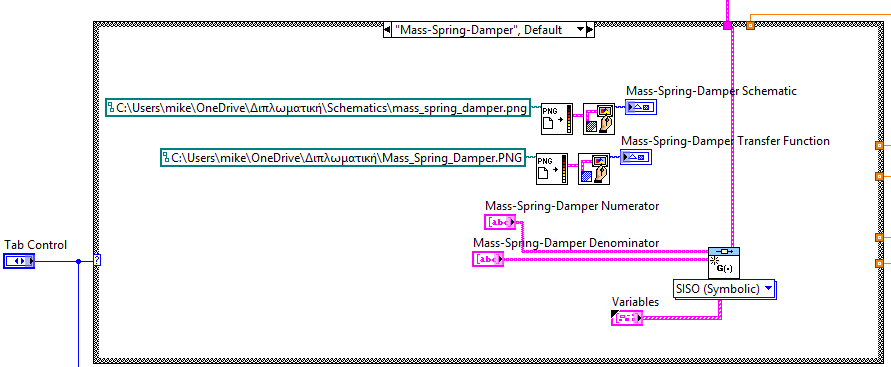
\includegraphics[width=\textwidth]{tab_controld}
  \caption{Block diagram του Tab Control}
  \label{fig:tab_controld}
\end{figure}

\begin{figure}[h]
  \centering
  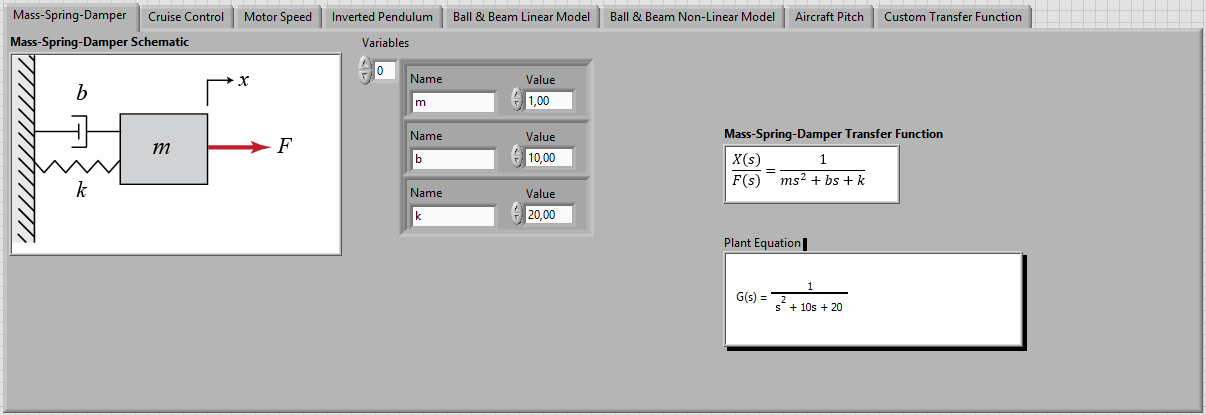
\includegraphics[width=\textwidth]{tab_controlp}
  \caption{Front panel του Tab Control}
  \label{fig:tab_controlp}
\end{figure}

\subsection{Simulation Loop}

Ο κύριος αλγόριθμος υλοποιείται μέσα στο μαύρο πλαίσιο του Σχήματος \ref{fig:simulation_loopd} και το οποίο ονομάζεται ``Simulation Loop". Η δομή αυτή παρέχεται από το ``Control and Simulation Toolkit" του LabVIEW. Στην ουσία αποτελεί μία επαναληπτική δομή η οποία έχει ενσωματωμένους αλγορίθμους για την επίλυση διαφορικών εξισώσεων. Το ``Simulation Loop" έχει πολλές επιλογές που ο χρήστης μπορεί να ρυθμίσει ανάλογα με τι θέλει να πετύχει. Για τις απαιτήσεις της εργασίας αυτής επιλέχθηκε οι διαφορικές εξισώσεις να επιλύονται με τον αλγόριθμο ``Runge-Kutta $4$" με σταθερό χρονικό βήμα step size $= 0.01$ seconds. Άρα κάθε $10$ milliseconds το πρόγραμμα μετατρέπει τη συνάρτηση μεταφοράς σε διαφορική εξίσωση και χρησιμοποιεί τη μέθοδο επίλυσης ``Runge Kutta $4$" για να υπολογίσει την απόκριση του συστήματος $y(t)$. Είναι προφανές, ότι πιο προχωρημένες μέθοδοι επίλυσης (πχ ``Runge Kutta $45$") θα οδηγήσουν σε μία, ενδεχομένως, πιο ακριβής τιμή της απόκρισης του συστήματος. Μετά από δοκιμές, η μέθοδος που επιλέχθηκε προσεγγίζει αρκετά ικανοποιητικά την απόκριση των συστημάτων, με τις διαφορές της σε σχέση με πιο προηγμένες μεθόδους να είναι ανεπαίσθητες.

Αφού ο χρήστης επιλέξει το σύστημα που θέλει να ελέγξει, πατάει το ``Run" και το πρόγραμμα αρχίζει την εκτέλεσή του. Αρχικά, εκτιμάται η συνάρτηση μεταφοράς με βάση τις αριθμητικές τιμές των παραμέτρων του συστήματος που έχει δώσει ο χρήστης. Στη συνέχεια αυτό το μοντέλο τροφοδοτείται στο ``Transfer Function.vi" που βρίσκεται μέσα στο simulation loop. Σε κάθε επανάληψη του simulation loop, το VI αυτό έχει σαν έξοδο την εκτίμηση της εξόδου που θα είχε το πραγματικό σύστημα.

\begin{figure}[h]
  \centering
  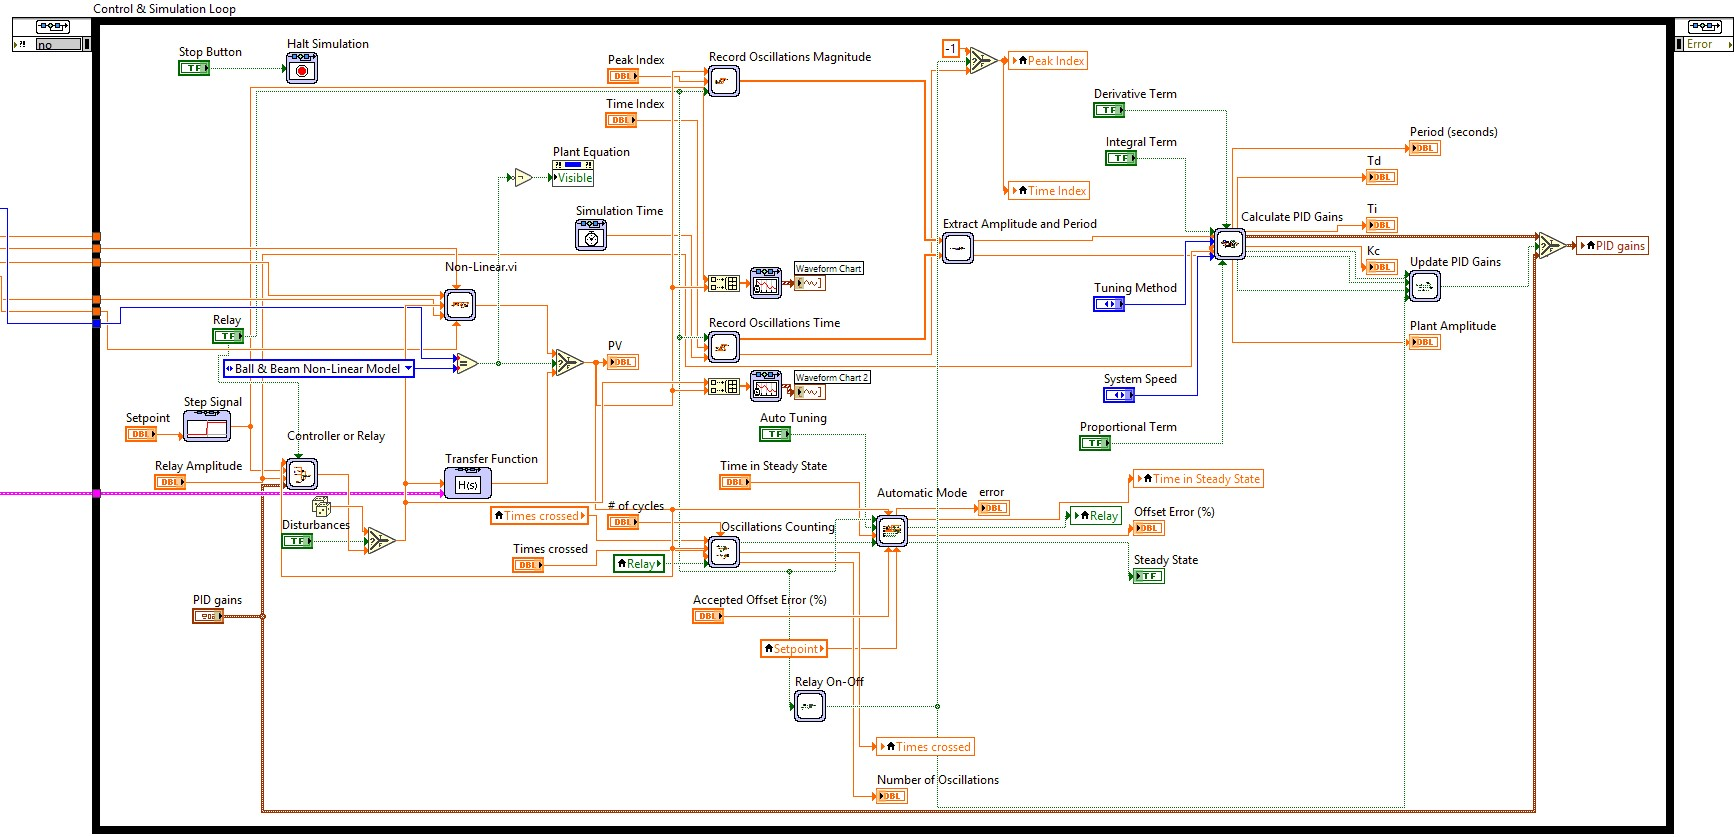
\includegraphics[width=\textwidth]{simulation_loopd}
  \caption{Το Simulation Loop}
  \label{fig:simulation_loopd}
\end{figure}

\subsection{Controller or Relay subVI}

Στο Σχήμα \ref{fig:Controller_or_Relayd} παρουσιάζεται το block diagram του subVI που αναλαμβάνει να αντικαταστήσει τον PID ελεγκτή με το relay στοιχείο έτσι ώστε να πραγματοποιηθεί το πείραμα. Το subVI αυτό δέχεται ως εισόδους την αριθμητική τιμή της εξόδου του συστήματος, την επιθυμητή τιμή (\emph{setpoint}) που θέλουμε να έχει το σύστημα, το πλάτος του τετραγωνικού παλμού relay, τα κέρδη του PID ελεγκτή (\emph{PID gains}) καθώς και ένα λογικό (\emph{boolean}) σήμα με το όνομα ``Relay". Το λογικό αυτό σήμα ενεργοποιείται είτε μετά από εντολή του χρήστη πατώντας το αντίστοιχο κουμπί στο front panel, είτε αυτόματα όταν ικανοποιηθούν κάποιες προϋποθέσεις που έχει θέσει ο χρήστης. Το λογικό αυτό σήμα τροφοδοτείται στη δομή ``Select". Αν η τιμή της λογικής μεταβλητής είναι \textit{True} τότε η δομή επιλέγει το πάνω σήμα που τροφοδοτείται σε αυτή, ενώ αν είναι \textit{False} επιλέγει το κάτω. Έτσι λοιπόν καθορίζεται το σήμα ελέγχου $u(t)$ που έπειτα τροφοδοτείται στο σύστημα. Αν δηλαδή το κουμπί ``Relay" είναι πατημένο ο διακόπτης στο Σχήμα \ref{fig:relay} βρίσκεται στην πάνω θέση, ενώ αν δεν είναι ο διακόπτης βρίσκεται στην κάτω θέση.

\begin{figure}[h]
  \centering
  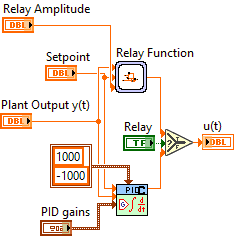
\includegraphics[width=\textwidth,height=5cm,keepaspectratio]{Controller_or_Relayd}
  \caption{Controller or Relay block diagram}
  \label{fig:Controller_or_Relayd}
\end{figure}

\subsubsection{Relay Function}

Όπως φαίνεται από το Σχήμα \ref{fig:Controller_or_Relayd}, μέσα στο ``Controller or Relay" subVI υπάρχει ένα ακόμα subVI με όνομα ``Relay Function". Το block diagram αυτού παρουσιάζεται στο Σχήμα \ref{fig:Relayd}. Η συνάρτηση αυτή δέχεται ως εισόδους το setpoint, την έξοδο του συστήματος και το πλάτος του relay. Στη συνέχεια αφαιρεί την έξοδο του συστήματος από το setpoint υπολογίζοντας το σφάλμα. Αν το σφάλμα είναι μεγαλύτερο από το setpoint τότε η έξοδος του relay (\emph{Relay Out}) είναι $+Relay \ Amplitude$ ενώ αν είναι μικρότερο από το setpoint η έξοδος είναι $-Relay \ Amplitude$.

\begin{figure}[H]
  \centering
  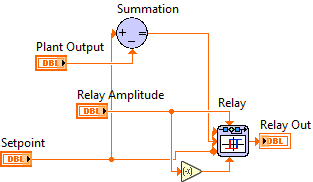
\includegraphics[width=\textwidth,height=5cm,keepaspectratio]{Relayd}
  \caption{Relay Function block diagram}
  \label{fig:Relayd}
\end{figure}

\subsection{Record Oscillations Magnitude subVI}

Όπως έχει ήδη αναφερθεί, προκειμένου να χρησιμοποιηθεί η μέθοδος για την αυτόματη ρύθμιση του PID ελεγκτή, θα πρέπει να μετρηθεί το πλάτος και η περίοδος των ταλαντώσεων του συστήματος όταν είναι συνδεδεμένο το relay στοιχείο στην είσοδο του. Προκειμένου να γίνεται καλύτερη διαχείριση μνήμης του προγράμματος και να μην πέφτει η απόδοσή του, τα δεδομένα της απόκρισης καταγράφονται μόνο όσο το λογικό σήμα ``Relay" έχει την τιμή \textit{True}. Το subVI αυτό είναι που αναλαμβάνει αυτή τη λειτουργία. Όσο λοιπόν το λογικό σήμα έχει αληθής τιμή, το subVI κάνει εισχωρεί με χρονολογική σειρά την αριθμητική τιμή της εξόδου του συστήματος $y(t)$ σε ένα πίνακα. Αυτός ο πίνακας, με όνομα ``Oscillations Magnitude Data", είναι η έξοδος του subVI. Όσο η τιμή του λογικού σήματος είναι μη αληθής, βάζει την τιμή NaN (\emph{Not a Number}). Τα δεδομένα αυτού του τύπου αγνοούνται από το LabVIEW και συνεπώς δεν έχουν επίδραση στη συνολική απόδοση του συστήματος.

\begin{figure}[h]
  \centering
  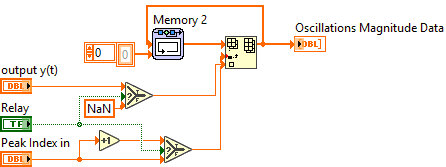
\includegraphics[width=\textwidth,height=5cm,keepaspectratio]{Record_Oscillations_Magnituded}
  \caption{Record Oscillations Magnitude block diagram}
  \label{fig:Record_Oscillations_Magnituded}
\end{figure}

\subsection{Record Oscillations Time subVI}

Το subVI αυτό λειτουργεί σε πλήρη αντιστοιχία με το προηγούμενο, με τη μόνη διαφορά ότι αυτό αντί να καταγράφει τις τιμές της απόκρισης του συστήματος, καταγράφει τις χρονικές στιγμές και τις βάζει στον πίνακα ``Oscillations Time Data". Όπως και πριν, αν η τιμή του ``Relay" είναι μη αληθής τότε στον πίνακα περνάει δεδομένα του τύπου NaN.

\begin{figure}[h]
  \centering
  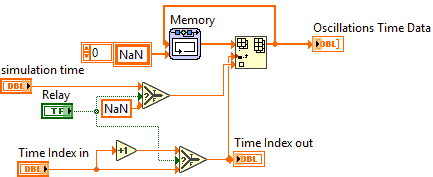
\includegraphics[width=\textwidth,height=5cm,keepaspectratio]{Record_Oscillations_Timed}
  \caption{Record Oscillations Time block diagram}
  \label{fig:Record_Oscillations_Timed}
\end{figure}

\subsection{Extract Amplitude and Period subVI}

Το συγκεκριμένο subVI είναι υπεύθυνο για τον υπολογισμό του πλάτους και της περιόδου των ταλαντώσεων. Ως εισόδους δέχεται τους πίνακες ``Oscillations Magnitude Data" και ``Oscillations Time Data" από τις δύο προηγούμενες συναρτήσεις. Αν, κατά την εκτέλεση του προγράμματος, το κουμπί ``Relay" πατηθεί πολλές φορές, το σύστημα θα εκτελέσει πολλά σετ ταλαντώσεων, ένα για κάθε ενεργοποίηση του ``Relay". Θα πρέπει λοιπόν το πρόγραμμα να είναι σε θέση να ξεχωρίσει το ένα σετ ταλαντώσεων από το άλλο. Για να γίνει αυτό ψάχνει στον πίνακα ``Oscillations Magnitude Data" για την τιμή NaN. Όπως αναφέρθηκε προηγουμένως, όταν η τιμή του ``Relay" είναι \textit{False}, στους πίνακες μπαίνει η τιμή αυτή. Οπότε παίζει το ρόλο του διαχωριστικού μεταξύ των ταλαντώσεων που οφείλονται σε ξεχωριστό πάτημα του κουμπιού ``Relay".

Αφού βρεθούν, τα δεδομένα που αντιπροσωπεύουν την ίδια ταλάντωση εισάγονται στο ``Peak Detector.vi" του LabVIEW το οποίο βρίσκει τα ακρότατα των δεδομένων καθώς και τις θέσεις του πίνακα που βρίσκονται αυτά τα ακρότατα. Σύμφωνα με τη θεωρία, το σύστημα εκτελεί ταλαντώσεις αμείωτου πλάτους, οπότε για να βρούμε το πλάτος, αρκεί να κρατήσουμε μία, οποιαδήποτε, από τις τιμές που μας δίνει ως ακρότατο το ``Peak Detector.vi". Επίσης, τα δεδομένα  στους πίνακες ``Oscillations Magnitude Data" και ``Oscillations Time Data" είναι εντελώς συμμετρικά. Δηλαδή, στη θέση του πίνακα που υπάρχει η τιμή του πλάτους της ταλάντωσης, στην ακριβώς ίδια θέση του πίνακα που περιέχει τις χρονικές στιγμές, θα υπάρχει η χρονική στιγμή κατά την οποία το σύστημα είχε το συγκεκριμένο πλάτος. Συνεπώς, για να βρούμε την περίοδο των ταλαντώσεων, το μόνο που χρειάζεται είναι να αφαιρεθούν οι χρονικές στιγμές δύο διαδοχικών μέγιστων ακρότατων.

\begin{figure}[h]
  \centering
  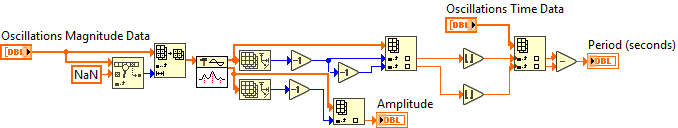
\includegraphics[width=\textwidth,height=5cm,keepaspectratio]{Extract_Amplitude_and_Periodd}
  \caption{Extract Amplitude and Period block diagram}
  \label{fig:Extract_Amplitude_and_Periodd}
\end{figure}

\subsection{Calculate PID Gains subVI}

Αφού έχουν βρεθεί τα χαρακτηριστικά των ταλαντώσεων, συγκεκριμένα το πλάτος και η περίοδος, το μόνο που απομένει είναι ο αριθμητικός υπολογισμός των παραμέτρων. Αυτό αναλαμβάνει να κάνει το συγκεκριμένο subVI. Το υποσύστημα δέχεται ως εισόδους το πλάτος του τετραγωνικού παλμού, το πλάτος των ταλαντώσεων, την περίοδο των ταλαντώσεων, τη μέθοδο ρύθμισης (Ziegler-Nichols ή Tyreus-Luyben) και την επιθυμητή ταχύτητα απόκρισης που θέλουμε να έχει το σύστημα μετά τον έλεγχο (ισχύει μόνο για τη μέθοδο Ziegler-Nichols). Στο Σχήμα \ref{fig:Calculate_PID_Gainsd_TL} έως και το Σχήμα \ref{fig:Calculate_PID_Gainsd_ZN_slow}, φαίνεται ο κώδικας κάθε περίπτωσης και πώς υπολογίζονται τα κέρδη. Αρχικά υπολογίζεται το απόλυτο κέρδος σύμφωνα με τον τύπο \ref{eq:Ku} και μετά ανάλογα με την τιμή που έχει το ``Tuning Method" υπολογίζονται οι τιμές των $K_p,\ T_i,\ T_d$. Οι τύποι για τον υπολογισμό των παραμέτρων συνοψίζονται στον πίνακα \ref{table:autotuning_parameters}. Μια μικρή λεπτομέρεια που αξίζει να αναφερθεί για αποφυγή μπερδεμάτων είναι ότι στον κώδικα, οι χρονικές παράμετροι $T_i$ και $T_d$ διαιρούνται με το $60$. Αυτό γίνεται επειδή το ``PID.vi" του LabVIEW που έχει χρησιμοποιηθεί στην εργασία δέχεται τις παραμέτρους σε λεπτά και όχι σε δευτερόλεπτα όπως έχουν υπολογιστεί αρχικά. 

\begin{table}[h]
\begin{center}
	\begin{tabular}{|c|c|c|c|c|}
	\hline 
	\textbf{Μέθοδος ελέγχου} & \textbf{Ταχύτητα} & $\mathbf{K_p}$ & $\mathbf{T_i}$ & $\mathbf{T_d}$ \\ 
	\hline 
	Tyreus-Luyben & -- & $K_u/2.2$ & $2.2T_u$ & $T_u/6.3$ \\ 
	\hline
	Ziegler-Nichols & Fast & $0.6K_u$ & $T_u/2$ & $T_u/8$ \\
	\hline
	Ziegler-Nichols & Normal & $0.33K_u$ & $T_u/2$ & $T_u/3$ \\
	\hline
	Ziegler-Nichols & Slow & $0.2K_u$ & $T_u/0.1$ & $T_u/0.8$ \\
	\hline
	\end{tabular} 
\caption{Τύποι για την αυτόματη ρύθμιση του ελεγκτή}
\label{table:autotuning_parameters}
\end{center}
\end{table}

Μετά τον υπολογισμό τους, τα κέρδη εισάγονται στη δομή ``PID Gains" που αποτελεί και την έξοδο του συστήματος. Προκειμένου να υπάρχει ομαλή εκτέλεση του προγράμματος, πριν ανανεωθούν τα κέρδη περνάνε από κάποιους υπολογισμούς. Έτσι, αρχικά, αν τα κουμπιά για την ενεργοποίηση του κάθε όρου είναι απενεργοποιημένα τότε το κέρδος αυτού του όρου θα είναι μηδέν. Εξαίρεση αποτελεί ο αναλογικός όρος ο οποίος όταν είναι απενεργοποιημένο το κουμπί του το κέρδος του είναι μοναδιαίο, δηλαδή έχει ελάχιστη έως μηδαμινή επίδραση στην απόκριση του συστήματος. Αν ήταν μηδέν, τότε στην έξοδο του συστήματος δε θα βλέπαμε τίποτα καθώς όλα τα κέρδη θα ήταν μηδέν.

\begin{figure}[h]
  \centering
  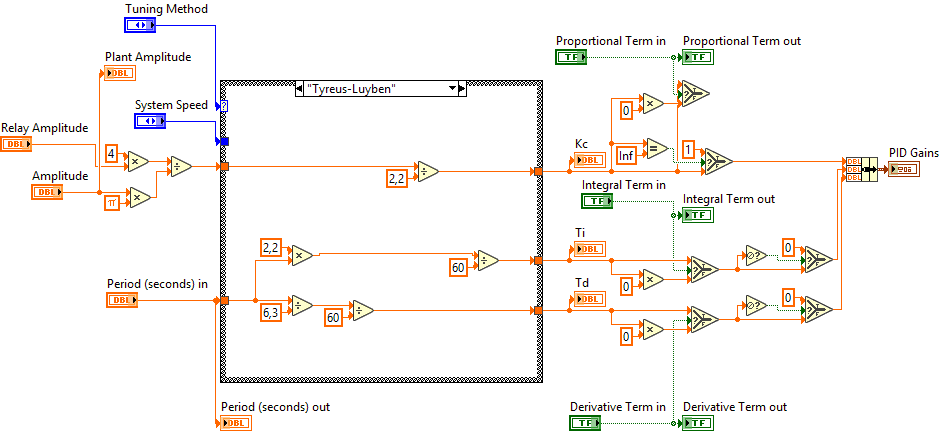
\includegraphics[width=\textwidth]{Calculate_PID_Gainsd_TL}
  \caption{Calculate PID Gains block diagram για την περίπτωση χρησιμοποίησης Tyreus-Luyben μεθόδου}
  \label{fig:Calculate_PID_Gainsd_TL}
\end{figure}

\begin{figure}[h!]
  \centering
  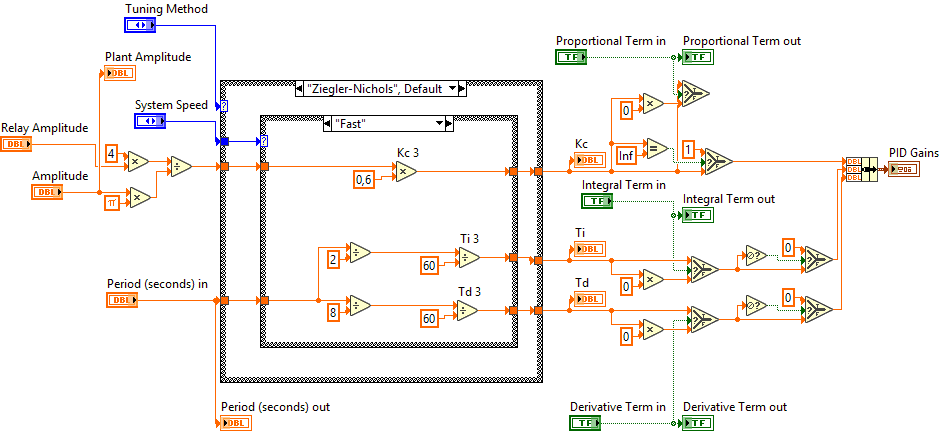
\includegraphics[width=\textwidth]{Calculate_PID_Gainsd_ZN_fast}
  \caption{Calculate PID Gains block diagram για την περίπτωση χρησιμοποίησης Ziegler-Nichols μεθόδου, γρήγορης ταχύτητας απόκρισης}
  \label{fig:Calculate_PID_Gainsd_ZN_fast}
\end{figure}

\begin{figure}[h]
  \centering
  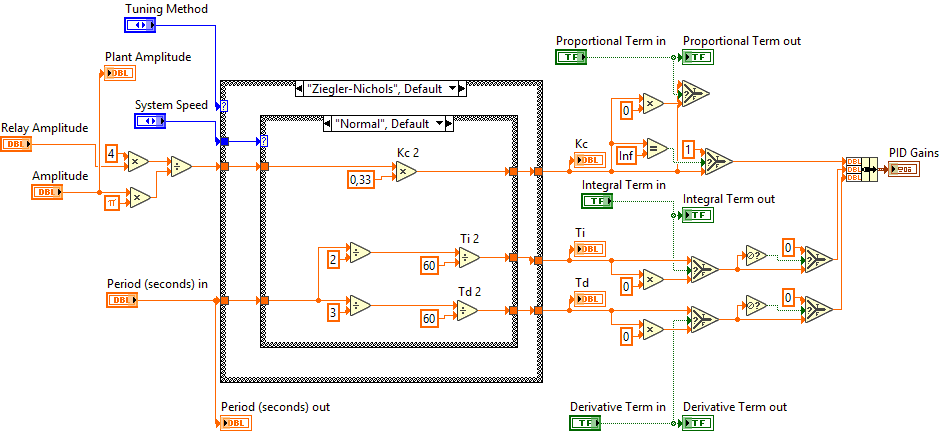
\includegraphics[width=\textwidth]{Calculate_PID_Gainsd_ZN_normal}
  \caption{Calculate PID Gains block diagram για την περίπτωση χρησιμοποίησης Ziegler-Nichols μεθόδου, μεσαίας ταχύτητας απόκρισης}
  \label{fig:Calculate_PID_Gainsd_ZN_normal}
\end{figure}

\begin{figure}[h!]
  \centering
  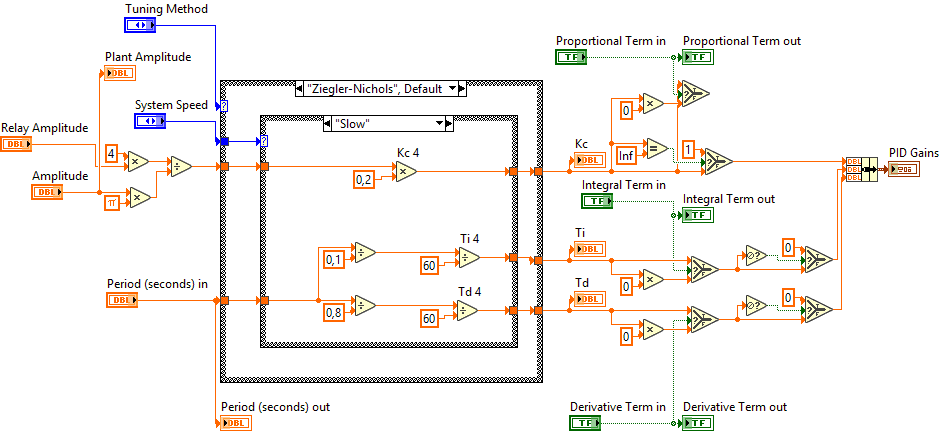
\includegraphics[width=\textwidth]{Calculate_PID_Gainsd_ZN_slow}
  \caption{Calculate PID Gains block diagram για την περίπτωση χρησιμοποίησης Ziegler-Nichols μεθόδου, αργής ταχύτητας απόκρισης}
  \label{fig:Calculate_PID_Gainsd_ZN_slow}
\end{figure}

Επίσης, σε κάθε επανάληψη του προγράμματος γίνεται έλεγχος για την τιμή που έχουν τα κέρδη. Αν οι τιμές τους δεν είναι κάποιος πραγματικός αριθμός αλλά κάποιου άλλου είδους δεδομένα, τότε η προσομοίωση του συστήματος θα αποτύχει και η απόκριση του συστήματος δε θα έχει σχέση με την πραγματική. Λόγω του τρόπου με τον οποίο έχει φτιαχτεί το πρόγραμμα, η προεπιλεγμένη τιμή για το αναλογικό κέρδος είναι άπειρο (\emph{Inf}) ενώ για τα άλλα δύο είναι το NaN. Ένας πραγματικός PID ελεγκτής όμως θα είχε ως αρχικά κέρδη τα $K_p = 1,\ T_i = 0,\ T_d = 0$. Συνεπώς, το πρόγραμμα ελέγχει το αναλογικό κέρδος αν έχει την τιμή \textit{Inf}. Αν αυτό ισχύει, τότε η τιμή του γίνεται μονάδα, αλλιώς ο αλγόριθμος κρατάει αυτή που έχει. Ομοίως, για τα άλλα δύο κέρδη, ελέγχει αν έχουν την τιμή NaN. Αν αυτό ισχύει τότε οι τιμές τους γίνονται μηδενικές ενώ σε αντίθετη περίπτωση διατηρούν αυτές που είχαν.

\subsection{Update PID Gains subVI}

Στο Σχήμα \ref{fig:Update_PID_Gainsd} φαίνεται το δομικό διάγραμμα του συγκεκριμένου υποσυστήματος. Αυτό το subVI δέχεται ως εισόδους τα λογικά σήματα που παράγονται από το πάτημα των κουμπιών ``Proportional Term", ``Integral Term", ``Derivative Term" και ``Relay". Τα σήματα αυτά περνάνε από κάποια άλλα επιμέρους subVIs τα οποία επιστρέφουν τιμή ``Αληθής" αν το λογικό σήμα έχει αλλάξει κατάσταση, δηλαδή εάν από ``Αληθής" η κατάστασή του έγινε ``Ψευδής" ή το αντίθετο και επιστρέφουν τιμή ``Ψευδής" αν το λογικό σήμα δεν έχει αλλάξει κατάσταση. Στο τέλος οι έξοδοι από τα υποσυστήματα αυτά περνάνε από μία πύλη που υλοποιεί τη λογική πράξη ``AND" και αποδίδουν μια τιμή στην έξοδο. Αν αυτή η τιμή είναι ``Αληθής" τότε τα κέρδη του ελεγκτή θα ανανεωθούν στις καινούριες τιμές, ενώ αν είναι ``Ψευδής" θα παραμείνουν ως έχουν. Εν συντομία, κάθε φορά που πατιέται είτε το κουμπί ``Relay" είτε κάποιο από τα κουμπιά των όρων του ελεγκτή, τα κέρδη ενημερώνονται έτσι ώστε η αλλαγή στην απόκριση να είναι άμεση χωρίς ο χρήστης να χρειάζεται να πατήσει κάποιο γενικό κουμπί ανανέωσης των κερδών.

\begin{figure}[h!]
  \centering
  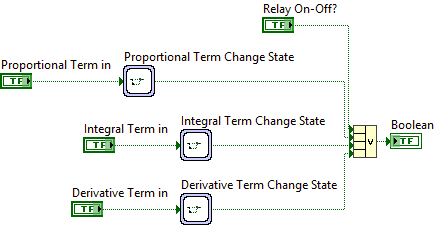
\includegraphics[width=\textwidth,height=5cm,keepaspectratio]{Update_PID_Gainsd}
  \caption{Update PID Gains block diagram}
  \label{fig:Update_PID_Gainsd}
\end{figure}

\subsection{Automatic Mode subVI}

Τα controls που φαίνονται στο Σχήμα \ref{fig:Automatic_Modef} αφορούν την αυτόματη λειτουργία του ελεγκτή. Το block diagram αυτής φαίνεται στο Σχήμα \ref{fig:Automatic_Moded}. Όταν το κουμπί ``Auto Tuning" είναι ενεργοποιημένο, τότε ο ελεγκτής ελέγχει αν το σύστημα βρίσκεται σε μόνιμη κατάσταση. Αν αυτό ισχύει, και το σφάλμα του συστήματος είναι μεγαλύτερο από αυτό που ο χρήστης έχει ορίσει ως επιτρεπτό σφάλμα μόνιμης κατάστασης (\emph{Accepted Offset Error \%)}, το κουμπί ``Relay" ενεργοποιείται αυτόματα. Ο ελεγκτής επανέρχεται σε λειτουργία όταν το σύστημα εκτελέσει τόσες ταλαντώσεις όσες έχει ορίσει ο χρήστης στο πεδίο ``\# of cycles". Προφανώς όσες περισσότερες ταλαντώσεις κάνει το σύστημα, τόσο πιο πιθανόν είναι αυτές να έχουν ξεπεράσει τα μεταβατικά φαινόμενα και να έχουν σταθερό πλάτος και περίοδο. Από τις δοκιμές που πραγματοποιήθηκαν φάνηκε ότι περίπου τρεις ταλαντώσεις είναι αρκετές για να επέλθει αυτή η κατάσταση.

Με την πάροδο του χρόνου, τα χαρακτηριστικά μιας διεργασίας μπορεί να αλλοιωθούν και να αλλάξουν ελαφρώς. Αυτό έχει ως αποτέλεσμα, ο έλεγχος που στο παρελθόν ήταν ικανοποιητικός πλέον να κρίνεται ανεπαρκής. Η λειτουργία ``Auto Tuning" αποσκοπεί στο να λύσει αυτό το πρόβλημα. Αν λοιπόν, για παράδειγμα, μια διεργασία στην οποία ο έλεγχος επέβαλλε μηδενικό σφάλμα μόνιμης κατάστασης αλλάξει και το σφάλμα πλέον έχει μια τιμή μεγαλύτερη από την αποδεκτή, ο ελεγκτής θα το αντιληφθεί και θα προσαρμοστεί αυτόματα στα καινούρια δεδομένα χωρίς την παρέμβαση του χρήστη.

\begin{figure}[h]
  \centering
  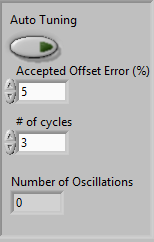
\includegraphics[width=\textwidth,height=5cm,keepaspectratio]{Automatic_Modef}
  \caption{Automatic Mode front panel}
  \label{fig:Automatic_Modef}
\end{figure}

\begin{figure}[h]
  \centering
  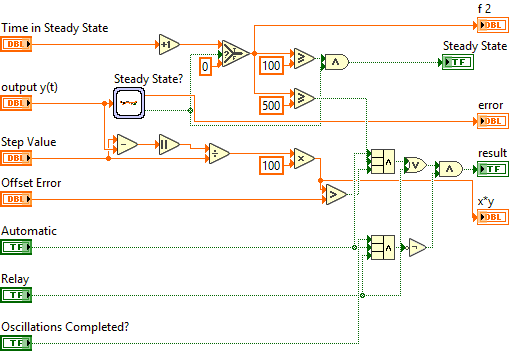
\includegraphics[width=\textwidth,height=5cm,keepaspectratio]{Automatic_Moded}
  \caption{Automatic Mode block diagram}
  \label{fig:Automatic_Moded}
\end{figure}

Προκειμένου το σύστημα να μην ανταποκρίνεται σε θόρυβο αλλά μόνο στο σφάλμα του συστήματος, αυτή η λειτουργία ενεργοποιείται μόνο άμα το σύστημα βρίσκεται σε μόνιμη κατάσταση για περισσότερο από πέντε δευτερόλεπτα. Προκειμένου να καταλαβαίνει ο ελεγκτής ότι η απόκριση του συστήματος έχει σταθεροποιηθεί, έχει υλοποιηθεί το υποσύστημα ``Steady State" που φαίνεται στο Σχήμα \ref{fig:Steady_Stated}. Η λογική του είναι αρκετά απλή. Ουσιαστικά ελέγχει αν η τρέχουσα αριθμητική τιμή της εξόδου του συστήματος διαφέρει κατά $0.0001$ από την προηγούμενη. Αν αυτό συμβαίνει τότε είναι ασφαλές να θεωρήσουμε ότι το σύστημα βρίσκεται σε μόνιμη κατάσταση και η έξοδος του subVI παίρνει την τιμή ``Αληθής". 

\begin{figure}[h]
  \centering
  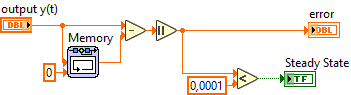
\includegraphics[width=\textwidth,height=5cm,keepaspectratio]{Steady_Stated}
  \caption{Steady State block diagram}
  \label{fig:Steady_Stated}
\end{figure}

\subsection{Oscillations Counting subVI}

Προκειμένου να ξέρει το πρόγραμμα πότε να σταματήσει τις ταλαντώσεις όταν η αυτόματη επιλογή είναι ενεργοποιημένη, θα πρέπει να είναι σε θέση να μετράει τις ταλαντώσεις που έχει εκτελέσει. Ο κώδικας που το κάνει αυτό φαίνεται στο Σχήμα \ref{fig:Oscillations_Countingd}. Οι ταλαντώσεις που εκτελεί το σύστημα κατά τη διάρκεια του πειράματος είναι συμμετρικές γύρω από το μηδέν. Συνεπώς, σε κάθε επανάληψη του προγράμματος και εφόσον το κουμπί ``Relay" είναι πατημένο, το subVI ελέγχει αν η έξοδος του συστήματος πέρασε την τιμή μηδέν πηγαίνοντας από τα αρνητικά στα θετικά. Κάθε φορά που αυτό συμβαίνει, αυξάνει την τιμή της μεταβλητής ``Times Crossed" κατά ένα. Αυτή η τιμή ισούται με την τιμή των ταλαντώσεων που έχει εκτελέσει το σύστημα. Επειδή οι πρώτες ταλαντώσεις δεν είναι σταθερές, με την έννοια ότι δεν έχουν σταθερό πλάτος, ο αλγόριθμος ξεκινάει το μέτρημα μετά από τις πρώτες δύο. Τέλος, όταν η λειτουργία ``Relay" απενεργοποιηθεί, είτε αυτόματα είτε από τον χρήστη, ο μετρητής επιστρέφει στο μηδέν.

\begin{figure}[h]
  \centering
  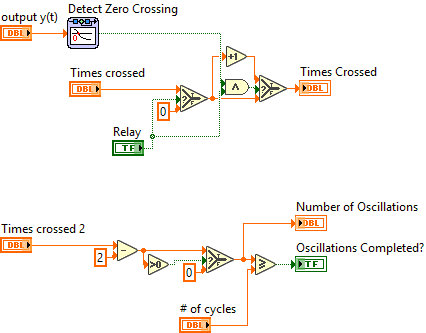
\includegraphics[width=\textwidth,height=5cm,keepaspectratio]{Oscillations_Countingd}
  \caption{Oscillation Counting block diagram}
  \label{fig:Oscillations_Countingd}
\end{figure}

\section{Σύνοψη}

Στο κεφάλαιο αυτό παρουσιάστηκε η θεωρία του αυτο-ρυθμιζόμενου PID ελεγκτή καθώς και η δομή του προγράμματος. Η λογική του κάθε υποσυστήματος αναλύθηκε εκτενώς και συμπεριλήφθηκαν εικόνες για την καλύτερη κατανόηση του κώδικα. Μετά από αυτό το κεφάλαιο, ο αναγνώστης θα πρέπει να έχει μια καλή ιδέα των αλγορίθμων του κάθε subVI καθώς και τον τρόπο που όλα μαζί συνδυάζονται προκειμένου να ``χτιστεί" το κυρίως πρόγραμμα. Στο επόμενο κεφάλαιο θα παρουσιαστούν τα πειράματα που έγιναν και τα συμπεράσματα σχετικά με την αποτελεσματικότητα του αυτο-ρυθμιζόμενου PID ελεγκτή.